\documentclass[12pt]{article}
\usepackage{amsmath} % For advanced math symbols
\usepackage{amsfonts} % For math fonts
\usepackage{amssymb} % Additional math symbols
\usepackage{geometry} % To adjust page margins
\usepackage{hyperref} % For clickable references
\usepackage{listings} % For displaying code files
\usepackage{parskip} % Skip paragraph indention
\usepackage{xcolor} % For colored links
\usepackage{graphicx}

% Page setup
\geometry{a4paper, margin=1in}
\hypersetup{
    colorlinks=true,
    linkcolor=blue,
    urlcolor=cyan,
}

\title{Investigation into Gaussian Quadrature}
\author{
    Jack Deye\\
    jackdeye@g.ucla.edu
    \and
    Zachary Diamond\\
    zacharydiamond@g.ucla.edu
    \and
    Jonathan Levi\\
    email@g.ucla.edu
    \and
    Reeshad Mohammed\\
    ree513@g.ucla.edu
}
\date{\today}

\begin{document}
\maketitle

\tableofcontents

\newpage

\section{Introduction}

Quadrature is the name given to various methods used to approximate integrals. Some integrals are
impossible or unfeasible to compute analytically (such as $\int e^{x^2}$), which necessitates the need to approximate them numerically.
Thus, various methods have been developed to approximate these integrals, such as the Trapezoid Rule, Simpson's Rule, and Gaussian Quadrature.
The aforementioned quadratures have varying levels of necessary computation and error. We intend to investigate and compare these quadrature forms.
In particular, we will analyze the accuracy of Gaussian Quadrature to the more simple Trapezoid Rule and Simpson's Rule.
Additionally, we will compare the theory of Guassian Quadrature convergence to experimental convergence.

\section{Quadrature Techniques}
\subsection{Trapezoid Rule}
The Trapezoid Rule is developed using Lagrange polynomials and equally spaced nodes. Consider $\int_a^b f(x)dx$. When we replace $f(x)$
with the first Lagrange polynomial approximation, with $x_0 = a$ and $x_1 = b$, and integrate, we get
\begin{align*}
	\frac{(x_1 - x_0)}{2}[f(x_0) + f(x_1)] - \frac{(x_1 - x_0)^3}{12}f''(\xi)
\end{align*}
Where $\xi \in (x_0, x_1)$. Naturally, we can set $h = x_1 - x_0$, resulting in the Trapezoid Rule:
\begin{align*}
	\int_{x_0}^{x_1}f(x)dx = \frac{h}{2}[f(x_0) + f(x_1)] - \frac{h^3}{12}f''(\xi)
\end{align*}
It is clear that this approach only works well on quite small intervals; so, we develop the Composite Trapezoid Rule. The Composite Trapezoid Rule
applies the Trapezoid Rule on $n$ subintervals within the initial interval. The formula is as follows:
\begin{align*}
	\int_{x_0}^{x_n}f(x)dx = \frac{h}{2}[f(x_0) + 2\sum_{j=1}^{n-1}f(x_j) + f(x_n)] - \frac{x_n - x_0}{12}h^2f''(\mu)
\end{align*}
Where $\mu \in (x_0, x_n)$.

\subsection{Simpson's Rule}
Similar to the Trapezoid Rule, Simpson's Rule is also developed using Lagrange polynomials. Simpson's Rule differs in that
it uses the second Lagrange polynomial. Consider $\int_{a}^{b} f(x)dx$. We set $x_0 = a$, $x_1 = a + h$, and $x_2 = b$, where $h = \frac{b - a}{2}$.
Now, when we replace $f(x)$ with the second Lagrange polynomial approximation and integrate, we get Simpson's Rule:
\begin{align*}
	\int_{x_0}^{x_2}f(x)dx = \frac{h}{3}[f(x_0) + 4f(x_1) + f(x_2)] - \frac{h^5}{90}f^{(4)}(\xi)
\end{align*}
Where $\xi \in (x_0, x_2)$. However, like the Trapezoid Rule, this form only works well on small intervals. The Composite Simpson's Rule is
developed similarly to the Composite Trapezoid Rule, splitting the interval into $n$ subintervals, where $n$ is an even integer.
The formula is as follows:
\begin{align*}
	\int_{x_0}^{x_n}f(x)dx = \frac{h}{3}[f(x_0) + 2\sum_{j=1}^{\frac{n}{2} - 1}f(x_{2j}) + 4\sum_{j=1}^{\frac{n}{2}}f(x_{2j - 1}) + f(x_n)] - \frac{x_n - x_0}{180}h^4f^{(4)}(\mu)
\end{align*}
Where $\mu \in (x_0, x_n)$.

\subsection{Guassian Quadrature}
Gaussian quadrature is particularly efficient for integrating polynomials and uses specially chosen points and weights to achieve high accuracy.

Gaussian quadrature approximates integrals using:
\[
	\int_a^b f(x) \, dx \approx \sum_{i=1}^n w_i f(x_i)
\]
where \( x_i \) are the nodes and $w_{i}$ are the weights.
The nodes and weights are chosen such that the method is exact for polynomials of degree $2n-1$ or lower.
Typically, this integral is from $[-1,1]$.

\subsubsection{Motivation}

Consider the trapezoid rule, which only provide exact solutions to integrals for linear functions.
But we can do better, take $n$ nodes $x_{1},x_{2},\cdots,x_{n}$. We can improve the trapezoid by choosing the weights such that they are exact for linear, quadratic, cubic, up to polynomials of degree $n-1$.\\
\begin{equation}
	\int_{-1}^{1}f \approx w_{1}f(x_{1})+w_{2}f(x_{2})+\cdots+w_{n}f(x_{n})
\end{equation}
\begin{align*}
	f(x)=1       & \to  \int_{-1}^{1}1 \,dx =  2 =            w_{1}+w_{2}+\cdot +w_{n}                                        \\
	f(x)=x       & \to  \int_{-1}^{1}x \,dx =  0 =            w_{1}x_{1}+w_{2}x_{2}+ \cdot +w_{n}x_{n}                        \\
	             & \vdots                                                                                                     \\
	f(x)=x^{n-1} & \to  \int_{-1}^{1}x^{n-1} \,dx =  0 =            w_{1}x_{1}^{n-1}+w_{2}x_{2}^{n-1}+\cdots+w_{n}x_{n}^{n-1} \\
\end{align*}
Resulting in the following linear equation (with a Vandermonde Matrix):
\[
	\begin{bmatrix}
		1           & 1           & \cdots & 1           \\
		x_{1}       & \ddots      & \cdots & x_{n}       \\
		\vdots      &             & \ddots &             \\
		x_{1}^{n-1} & x_{2}^{n-1} & \cdots & x_{n}^{n-1}
	\end{bmatrix}
	\begin{bmatrix}
		w_{1} \\ w_{2} \\ \vdots \\ w_{n}
	\end{bmatrix}
	=
	\begin{bmatrix}
		2 \\ 0 \\ \vdots \\ b_{i}
	\end{bmatrix}
\]
In practice, this method is not feasible because Vandermonde matrices are badly ill-conditioned, as the condition number increases exponentially, (https://arxiv.org/abs/1504.02118), resulting in slight changes in $b$ causing large changes in $w_{i}$'s.

\subsubsection{Derivation}

We develop the formula for Gaussian quadrature using Legendre Polynomials - a series of orthogonal polynomials obtained by performing the Gram-Schmidt process
on the standard basis for polynomials of degree $n$ and the inner product $\langle p,q \rangle = \int_{-1}^{1} p(x)q(x)\,dx$.
The first few Legendre Polynomials are as follows:
\begin{align*}
	L_{0}(x)= & 1                     \\
	L_{1}(x)= & x                     \\
	L_{2}(x)= & \frac{1}{2}(3x^{2}-1) \\
	          & \vdots
\end{align*}
Note that $L_i(x)$ is orthogonal to all polynomials of degree less than $i$, meaning $\forall p \in \mathbb{P}$, $\langle L_i, p \rangle$ for $\deg(p) \leq i$.
Importantly, they also have exactly $n$ roots over $\mathbb{R}$.\\

Now, given a polynomial $p(x)$ of degree $2n - 1$, we can divide it by $L_n$, resulting in the following division with degrees:
\begin{equation}
	\overbrace{p(x)}^{2n-1}=\overbrace{q(x)}^{n-1} \overbrace{L_{n}(x)}^{n}+\overbrace{r(x)}^{n-1}
\end{equation}
Integrating both sides, we get
\[
	\int_{-1}^{1}p(x) \,dx = \int_{-1}^{1}q(x) L_{n}(x)\,dx + \int_{-1}^{1}r(x)\,dx  = 0+\int_{-1}^{1}r(x) \,dx
\] because the orthogonality of $L_{n}(x)$. \\
Going back to quadrature, we can ensure the same behavior by picking nodes at the zeros of $L_{n}(x)$. \\
Because $\int_{-1}^{1} p(x)\,dx = \int_{-1}^{1}r(x)\,dx$, we can interpolate $r(x)$ exactly with Lagrange polynomials, resulting in
\[
	\int_{-1}^{1}r(x)\,dx = \int_{-1}^{1}\left( \sum_{i=1}^{n}f(x_{i})l_{i}(x)\right)\,dx = \sum_{i=1}^{n}f(x_{i})\int_{-1}^{1}l_{i}(x)\,dx
\]
meaning we choose our weights the be the integral of the Lagrange basis polynomials, or
\[
	w_{i}=\int_{-1}^{1}\prod_{{j=1 \\j \ne i}}^{n} \frac{x-x_{j}}{x_{i}-x_{j}}\,dx
\]
This results in perfect interpolation of polynomials of degree $2n-1$, with $n$ nodes.
We can relate Lagrange and Legendre polynomials and then use the Christoffel-Darboux formula to rewrite the definition of the weights as
\begin{equation}
	w_{i}=\frac{2}{(1-x_{i}^2)(L_{n}'(x_{i}))^{2}}
\end{equation}

Before using Gaussian Quadrature on any function, one must change an integral over $[a,b]$ to one over $[-1,1]$. This can be done with
\begin{equation*}
	\int_{a}^{b} f(x) \,dx = \int_{-1}^{1}f \left(\frac{b-a}{2}x+\frac{a+b}{2}\right)\frac{b-a}{2} \,dx
\end{equation*}
Resulting in a formula of:
\begin{equation}
	\int_{a}^{b}f(x) \approx \frac{b-a}{2}\sum_{i=1}^{n}w_{i}f \left(\frac{b-a}{2}x_{i}+\frac{a+b}{2} \right)
\end{equation}

\section{Error Estimate and Theoretical Convergence}
For order of convergence, we will begin with some theoretical results.
\\
\subsection{Properties of Gaussian-Legendre Polynomials}

In order to prove the error estimate for Gaussian-Legendre Polynomials, we need to use the properties below, which are in the Brief Overview and Developing Gaussian Quadrature sections. Note that Gaussian-Legendre Polynomials have the conditions that $[a, b] = [-1, 1]$, so the below is the Gaussian-Legendre approximation.
\begin{equation}
    \int_a^b f(x) \, dx \approx \sum_{i=1}^n w_i f(x_i)
\end{equation}
We will denote the right hand side approximation as $G(f)$. 
We will also use the fact that the weights, $w_i$, are the integral of the Lagrangian from a to b, which is -1 to 1, which was shown in the Developing Gaussian Quadrature Section.
\begin{equation}
    w_{i}=\int_{-1}^{1}\prod_{{j=1 \\j \ne i}}^{n} \frac{x-x_{j}}{x_{i}-x_{j}}\,dx
\end{equation}


\subsection{Gaussian-Legendre Quadrature Error Estimate}

Let $P_n(x)$ denote the Legendre polynomial of degree n. Let $x_i$ for $i = 1,\dots,n$ be the roots of $P_n(x)$. \\
We will prove the following.
Let $f \in C^{2n}[-1,1]$. Then there exists $c \in (-1,1)$ such that
\begin{equation}
    \int_{-1}^{1} f(x)dx = G(f) + \frac{f^{(2n)}(c)}{(2n)!}\int_{-1}^{1} P_n^2(x)dx,
\end{equation}
where G(f) is
\begin{equation}
    G(f) = \sum_{i=1}^n w_i f(x_i)
\end{equation}
Notice that G(f) is the same as in the section above.


\begin{proof}
We will use Hermite polynomials to justify the error estimate for Gaussian quadrature. Let $H_{2n-1}(x)$ denote a polynomial of degree $2n - 1$ such that
\begin{align*}
    H_{2n-1}(x_i) &= f(x_i) \\
    H'_{2n-1}(x_i) &= f'(x_i)
\end{align*}
From Hermite interpolation, we know such polynomial exists and is unique.
The difference between $f(x)$ and a Hermite polynomial $H_{n}(x)$ is 
\begin{equation}
    f(x) = H_{n}(x) + \frac{f^{(n+1)}(\xi(x))}{(n)!} \prod_{i=1}^{m}(x - x_i)^{k_i}.
\end{equation}
for some $\xi(x) \in (a, b)$, where n is the degree of the Hermite polynomial, m is the number of $x_i$ and ${k_i}$ is the known number derivatives of ${x_i}$ for $i = 1, \dots, n$ \\
For $H_{2n-1}(x)$, we know two derivatives at each $x_i$ for $i = 1, \dots, n$, so $k = 2$, and the following holds for some $\xi(x) \in (a, b)$
\begin{equation}
    f(x) = H_{2n-1}(x) + \frac{f^{(2n)}(\xi)}{(2n)!} \prod_{i=1}^{n}(x - x_i)^2
\end{equation}
We can see that $(x - x_1)\dots(x - x_n)$ is $P_n(x)$ with roots $x_i$ for $i \in 1,\dots,n$. So taking the integral from -1 to 1 of the equation above yields
\begin{equation}
    \int_{-1}^{1} f(x)dx = \int_{-1}^{1} H_{2n-1}(x)dx + \int_{-1}^{1}\frac{f^{(2n)}(\xi)}{(2n)!} P_n^2(x)dx
\end{equation}
From the 2n-1 degree precision of the Gaussian Quadrature, we get the following
\begin{equation}
    \int_{-1}^{1} H_{2n-1}(x)dx = G(H_{2n-1})
\end{equation}
Then using the definition of G, we get
\begin{equation}
    G(H_{2n-1}) = \sum_{i=1}^{n} H_{2n-1}(x_i)
\end{equation}
Lastly, since $H_{2n-1}(x)$ interpolates $f(x)$, the following summation holds
\begin{equation}
   \sum_{i=1}^{n} H_{2n-1}(x_i) = \sum_{i=1}^{n} f(x_i) = G(f).
\end{equation}
Combining the previous three equations yields
\begin{equation}
    \int_{-1}^{1} H_{2n-1}(x)dx = G(f)
\end{equation}
Since $P_n^2(x)$ is nonnegative, we can use Mean Value Theorem to conclude
\begin{equation}
    \int_{-1}^{1} \frac{f^{(2n)}(\xi(x))}{(2n)!} P_n^2(x)dx = \frac{f^{(2n)}(c)}{(2n)!} \int_{-1}^{1} P_n^2(x)dx
\end{equation}
for some $c \in (-1,1)$. 
\\
Substituting the right hand sides of the two equations above, we can conclude
\begin{equation}
    \int_{-1}^{1} f(x)dx = G(f) + \frac{f^{(2n)}(c)}{(2n)!}\int_{-1}^{1} P_n^2(x)dx
\end{equation}
completing the proof.

\end{proof}

\subsection{Implications of Error Estimate on When To Use Gaussian Quadrature}
As we can see from the error estimate, Gaussian-Legendre Quadrature has a strong order of convergence as sene with the inclusion of the factorial term that grows quickly as well as the integral of the squared Legendre- polynomial having a strong order of convergence. 
\\
\\
The main conditions are $f \in C^{2n}[-1,1]$ and the integral being from -1 to 1.
\\
\\
The proof above generalizes to Gaussian Quadrature on [a,b], so the second condition is not much of an issue with the following result where w(x) is no longer equal to 1.
\\
\\
Note that the $P_n(x)$ used below is more restrictive than the Legendre polynomial. For more robust analysis on this general form, see page 22 of this source on page 22:
\\
(https://www.math.umd.edu/~mariakc/AMSC466/LectureNotes/quadrature.pdf)

\begin{equation}
    \int_a^b f(x)w(x)dx = Q(f) + \frac{f^{(2n)}(c)}{(2n)!} \int_a^b p_n^2(x)w(x)dx
\end{equation}
Then it follows in general that the extremely strong order of convergence for Gaussian Quadratures, including Gaussian-Legendre Quadratures, can be taken advantage of as long as we have highly smooth functions.
\\
\\
In the experimental section, we will try a variety of functions to see how Gaussian Quadrature performs relative to other Quadratures such as Trapezoidal Rule.
\\
\\
Based on the theoretical results above, for smooth functions, we should see Gaussian Quadrature dominates most quadratures.


\section{Comparison of Quadrature}

% \subsection{Composite Trapezoid Rule MATLAB Code}

% \lstinputlisting[language=Matlab]{composite_trapezoid_rule.m}

% \subsection{Composite Simpson's Rule MATLAB Code}

% \lstinputlisting[language=Matlab]{composite_simpsons_rule.m}

% \subsection{Gauss-Legendre Quadrature MATLAB Code}

% \lstinputlisting[language=Matlab]{gauss_legendre_quadrature.m}
% \lstinputlisting[language=Matlab]{GW_nodes_weights.m}
\begin{figure}[htbp]
	\begin{minipage}[b]{0.45\textwidth}
		\centering
		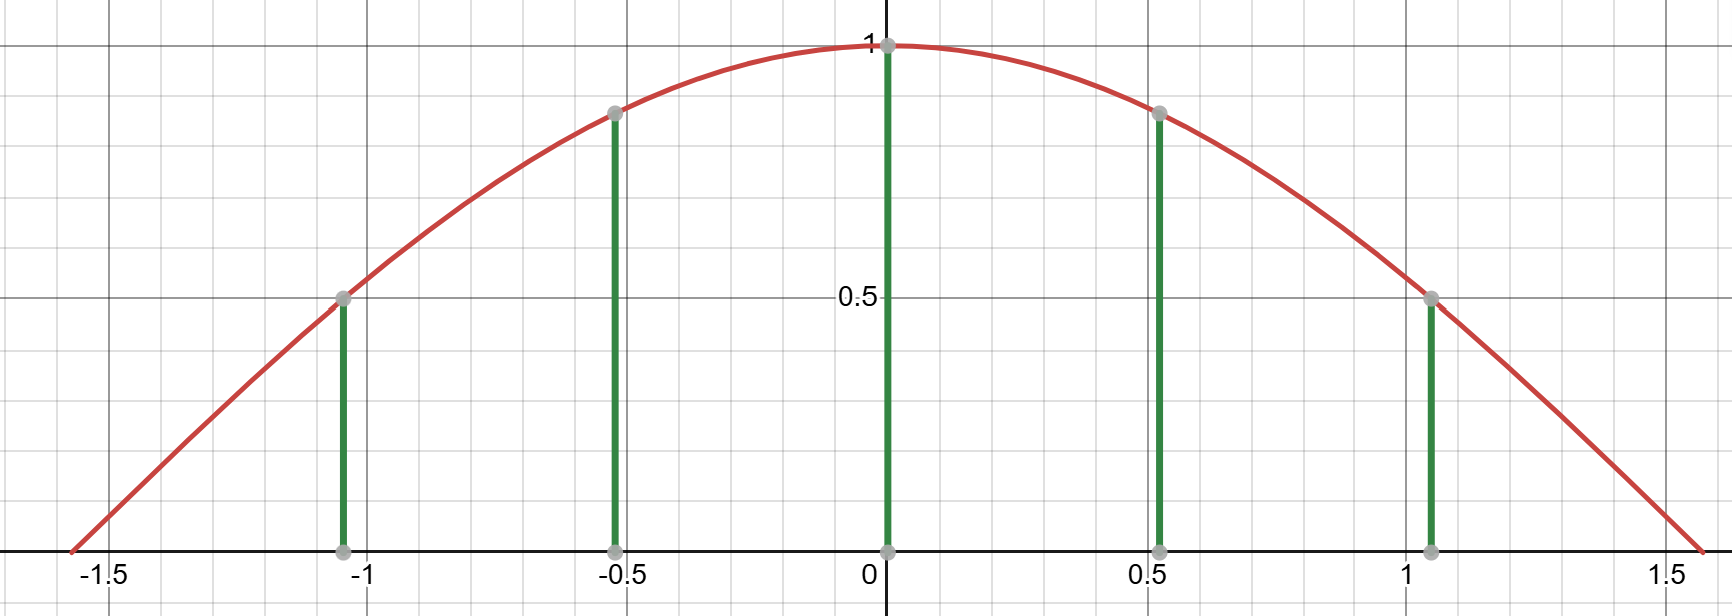
\includegraphics[width=\textwidth]{../images/Evenly_spaced.png} % Replace with the path to your first image
		\caption{Simpson and Trapezoid, evenly spacing for $\cos x$}
	\end{minipage}
	\hfill
	\begin{minipage}[b]{0.45\textwidth}
		\centering
		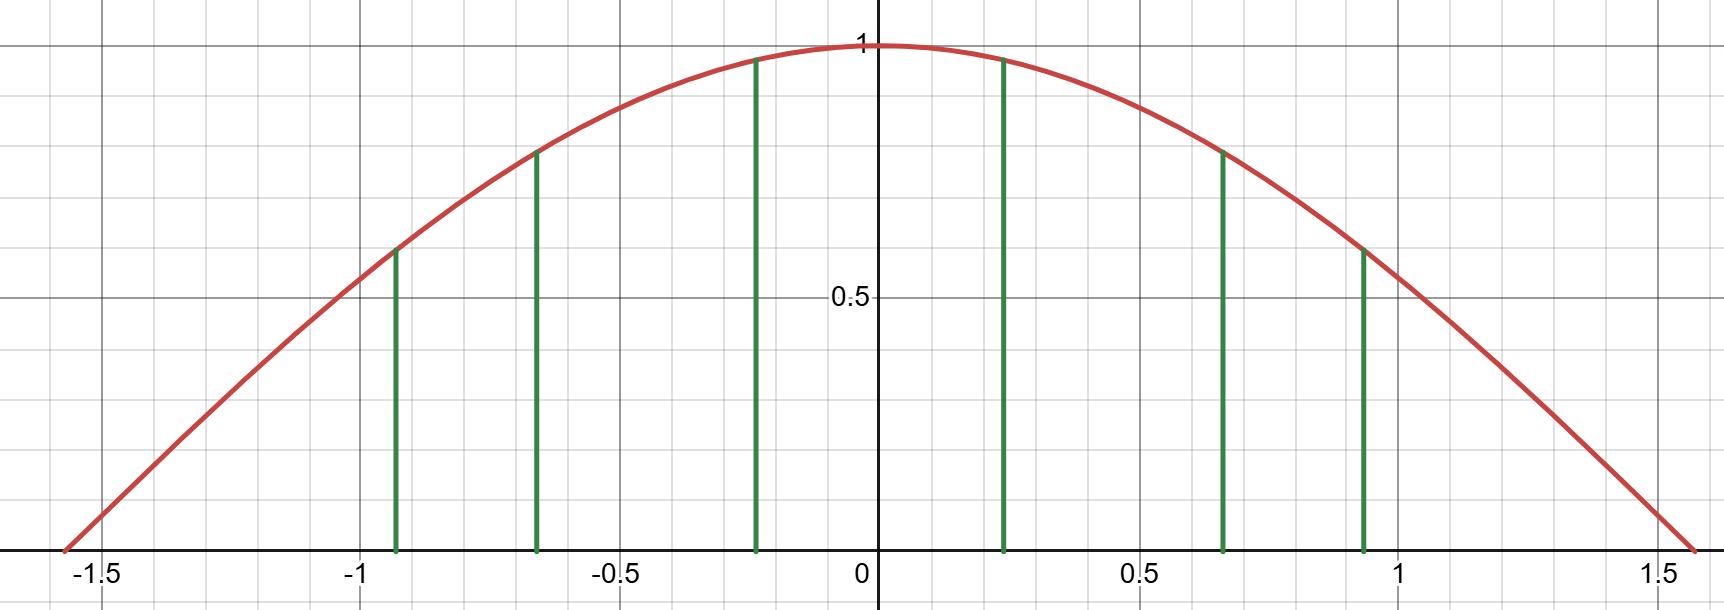
\includegraphics[width=\textwidth]{../images/GuassianQuad.png} % Replace with the path to your second image
		\caption{Gauss-Legendre node spacing, for $\cos x$}
	\end{minipage}
\end{figure}

We applied Trapezoid Rule, Simpson's Rule, and Gaussian Quadrature to a series of five functions for the purpose of
analysing and comparing the approximations. For each quadrature and function, we calculated the difference between
the approximation and the analytical solution, as well as the order of convergence. Below is a table of our results.

\begin{center}
	\begin{small}
		\begin{tabular}{| l | l | p{25mm} | p{17mm} | p{35mm} |}
			\hline
			Function & Method              & Final Absolute Error      & Terminated Early & Order of Convergence \\
			\hline
			F1       & Trapezoid Rule      & $3.88475 \times 10^{-7}$  & No               & Non-Polynomial       \\
			\hline
			F1       & Simpson's Rule      & $2.33869 \times 10^{-5}$  & No               & $O(n^{2.32})$        \\
			\hline
			F1       & Gaussian Quadrature & $7.56489 \times 10^{-6}$  & No               & Non-Polynomial       \\
			\hline
			F2       & Trapezoid Rule      & N/A                       & N/A              & N/A                  \\
			\hline
			F2       & Simpson's Rule      & N/A                       & N/A              & N/A                  \\
			\hline
			F2       & Gaussian Quadrature & $0.348133$                & No               & $O(n^{0.79})$        \\
			\hline
			F3       & Trapezoid Rule      & $0.0015914$               & No               & $O(n^{1.22})$        \\
			\hline
			F3       & Simpson's Rule      & $0.000641819$             & No               & $O(n^{1.59})$        \\
			\hline
			F3       & Gaussian Quadrature & $0.000938918$             & No               & $O(n^{1.21})$        \\
			\hline
			F4       & Trapezoid Rule      & $6.51042 \times 10^{-6}$  & No               & $O(n^{1.69})$        \\
			\hline
			F4       & Simpson's Rule      & $3.77476 \times 10^{-14}$ & No               & $O(n^{5.66})$        \\
			\hline
			F4       & Gaussian Quadrature & $0$                       & $n = 14$         & $O(n^{11.36})$       \\
			\hline
			F5       & Trapezoid Rule      & $0.000257028$             & No               & $O(n^{1.70})$        \\
			\hline
			F5       & Simpson's Rule      & $-2.64288 \times 10^{-8}$ & No               & $O(n^{3.45})$        \\
			\hline
			F5       & Gaussian Quadrature & $0$                       & $n = 12$         & $O(n^{13.02})$       \\
			\hline
		\end{tabular}
	\end{small}
\end{center}

\begin{align*}
	 & \text{Integrals:}                                                                                                         \\
	 & \text{F1: }f(x) = \frac{1}{1 + 1000(x - 0.5)^2}, \quad [0, 1]                                                             \\
	 & \text{F2: }f(x) = \frac{1}{x}\sqrt{\frac{1 + x}{1 - x}}\ln\left(\frac{2x^2 + 2x + 1}{2x^2 - 2x + 1}\right), \quad [-1, 1] \\
	 & \text{F3: }f(x) = \sqrt{|x|}, \quad [-1, 1]                                                                               \\
	 & \text{F4: }f(x) = \frac{1}{1 + x^2}, \quad [0, 1]                                                                         \\
	 & \text{F5: }f(x) = \cos(x), \quad [-\frac{\pi}{2}, \frac{\pi}{2}]
\end{align*}

\section{Experimental Order of Convergence}

\subsection*{Comparing Gaussian Quadrature to Trapezoidal Rule and Simpsons Rule}
Using the functions and results from section 3 directly above,  we will analyze how Gaussian Quadrature performed.

\subsubsection{Function 1}

As seen in the table, Function 1 based on performance by order of convergence has Trapezoid Rule $>$ Gaussian Quadrature $>$ Simpson's Rule. This case has a unique non-polynomial order of convergence for Trapezoid and Gaussian Quadrature. This means that they do not have the form of $O(n^m)$, where m is a real number. In this case, we can look at the log graph below. 

\begin{figure}
    NEED TO ADD THE FIGURE
\end{figure}

The main thing to notice is that the log graph does not appear linear or constant, and as such, this means a polynomial form does not fit. It does not conform to any type of pattern that aligns with a $O(n^m)$ form, but we can see that the Gaussian Quadrature did perform well based on the error being better than Simpson's Rule. This suggests that the non-polynomial order of convergence is still strong in this case and at least beats out $O(n^{2.32})$, so it is better than at least some polynomial order of convergences.

Trapezoid Rule performing better than Gaussian Quadrature is surprising to see in the errors, but this anomaly makes sense due to the function not conforming to neatly polynomial based integration.

\subsubsection{Function 2}

For Function 2, the property of the function leads to a division by zero preventing the use of Trapezoid and Simpson Rules. This is a situation where Gaussian Quadrature shines as it does not run into this issue due to the formulation; hence, it can still compute the integral. 

This function is also the worst type of Gaussian Quadrature performance since it only exhibits a close to linear order of convergence. Considering Gaussian Quadrature performs well when functions are smooth, this makes sense as Function 2 is not continuous, which is easily seen with the $\frac{1}{x}$ term.

\subsubsection{Function 3}

In this case, Gaussian Quadrature performed worse than Simpson's Rule, but beat Trapezoid Rule as seen by the errors in the table. This shows that in some cases Simpson's Rule can be quite effective, especially when smoothness does not hold, and there is low differentiability. In this case, the absolute value leads to non-differentiability at $x = 0$, which is in the interval of interest.

\subsubsection{Function 4}

This case shows why Gaussian Quadrature is powerful as the error is 0, meaning it is lower than machine epsilon, which is $2^{-52}$ for context. This aligns with the exactness of Gaussian Quadrature on highly differentiable polynomials property seen in the theoretical results. This is much better than Trapezoid and Simpson's Rules as well. The termination is also in 14 iterations, which is impressive.

\subsubsection {Function 5}

Here is another situation where Gaussian Quadrature properties lead to zero error, beating out machine epsilon once again. An impressive iteration count of 12 was also achieved to termination. This demonstrates once again how smooth functions with strong polynomial approximations, which is true due to the Taylor expansion of cosine, yields exact results. We should also note that in this case, we are extending outside of the Legendre polynomials as the interval includes values outside -1 and 1.

\section{Conclusion}

Overall, Gaussian Quadrature is a powerful method for integral approximation. It can compete with other quadratures such as Trapezoid and Simpson's, often out-performing them due to its impressive order of convergence as seen in the proof of error estimates. The main drawbacks are for cases where functions are not approximated well as polynomials, which leads to poor results. Outside of that, Gaussian Quadrature is able to yield a result when there is division by zero issues for other quadratures and can still get an average estimate even with a few discontinuities. One of the best features of Gaussian Quadrature is exactness for polynomials based on differentiability. This means that functions with strong polynomial approximations, which are smooth are guaranteed to have highly precise estimates over short iteration counts. Simply put, the exactness property of Gaussian Quadratures make it an excellent choice for approximating integrals, especially with high differentiability and close polynomial approximations.




\section{Conclusion}

Overall, Gaussian Quadrature is a powerful method for integral approximation. It can compete with other quadratures such as Trapezoid and Simpson's, often out-performing them due to its impressive order of convergence as seen in the proof of error estimates. The main drawbacks are for cases where functions are not approximated well as polynomials, which leads to poor results. Outside of that, Gaussian Quadrature is able to yield a result when there is division by zero issues for other quadratures and can still get an average estimate even with a few discontinuities. One of the best features of Gaussian Quadrature is exactness for polynomials based on differentiability. This means that functions with strong polynomial approximations, which are smooth are guaranteed to have highly precise estimates over short iteration counts. Simply put, the exactness property of Gaussian Quadratures make it an excellent choice for approximating integrals, especially with high differentiability and close polynomial approximations.

\newpage
\section{References}

\begin{enumerate}
	\item "https://www.math.umd.edu/~mariakc/AMSC466/LectureNotes/quadrature.pdf", page 22 error estimates
	\item Numerical Analysis, Richard L. Burden, J. Douglas Faires, etc.
\end{enumerate}


\end{document}
